%%%%%%%%%%%%%%%%%%%%%%%%%%%%%%%%%%%%%%%%%%%%%%%%%%%%%%%%%%%%%%%%%%%%
%%%%% DOC ARCHITECTURE : FONCTIONNEMENT DE LA PLATEFORME 	   %%%%%
%%%%%%%%%%%%%%%%%%%%%%%%%%%%%%%%%%%%%%%%%%%%%%%%%%%%%%%%%%%%%%%%%%%%

Le fonctionnement de la plateforme est directement lié au fonctionnement des classes implémentant l'interface \texttt{interfaces.IPluginManager} qui sont exécutées. Ce document ayant pour but d'expliquer le fonctionnement de l'implémentation actuelle, cette partie illustrera le comportement de la classe \texttt{pluginManager.PluginManager} fournie. Il est cependant tout à fait possible de créer une classe gérant les plugins d'une façon complètement différente de celle-ci, tant qu'elle respecte l'interface nécessaire pour être reconnue comme telle.

\section{Fonctionnement général}

Lors de son instanciation, la classe \texttt{pluginManager.PluginManager} lit son fichier de configuration (\textit{GestionnairePlugins/resources/init}) et enregistre son contenu. Ce contenu est ensuite analysé afin de récupérer les éléments suivants:\\

\begin{itemize}
	\item Le chemin commun vers tous les fichiers à charger ultérieurement.
	\item Les dossiers dans lesquels se trouvent les fichiers \texttt{.class} contenant les classes à charger. Les URLs de ces dossiers sont ensuite récupérées et passées en argument à l'\texttt{URLClassLoader} qui chargera toutes les classes utilisées.\\
\end{itemize}

Ces informations sont mémorisées par le gestionnaire de plugins, afin de pouvoir les transmettre aux plugins en ayant besoin.\\

Une fois ces actions effectuées, le gestionnaire effectue un scan de l'arborescence des dossiers gérés par l'\texttt{URLClassLoader} créé précédemment. Ce scan permet de trouver les fichiers \texttt{.class} contenant des plugins valides. Ces plugins sont mémorisés et classés selon leur type, qui est obtenu par l'appel à leur implémentation de la méthode \texttt{public String type()} de l'interface \texttt{interfaces.IPlugin}. L'inconvénient de cette façon d'obtenir le type est qu'elle nécessite d'instancier temporairement chaque plugin, ce qui peut être problématique suivant leur implémentation.\\

Une fois ce scan fini, le gestionnaire de plugins affiche dans la console qui l'a exécuté la liste des plugins disponibles classés par type, afin que l'utilisateur en prenne connaissance.\\

Le gestionnaire charge ensuite tous les plugins demandés dans le fichier de configuration, en leur fournissant le fichier de configuration associé. Si le plugin en question est un plugin complexe, le gestionnaire lui fourni également une référence vers son instance, afin que le plugin puisse demander le chargement des plugins dont il aura besoin.

\section{Fonctionnement spécifique : chargement d'un plugin}

\subsection{Chargement d'un plugin précis}

Le chargement d'un plugin est effectué par un appel à la méthode \texttt{public IPlugin loadPlugin(String pluginName, String initPath)} déclarée dans l'interface \texttt{IPluginManager}. Les deux arguments requis sont le nom complet de la classe à charger, et le chemin vers le dossier contenant le fichier d'initialisation associé.\\

Le gestionnaire commence par récupérer les informations contenues dans le fichier d'initialisation, auxquelles il ajoute les clefs \textit{pathToInit} et \textit{pathToHome} contenant respectivement le chemin vers le fichier d'initialisation (au cas où le plugin ait besoin d'analyser son contenu à nouveau) et le chemin vers l'arborescence commune à tous les éléments gérés par la plateforme (afin de fournir un point de départ pour accéder à un fichier).\\

La classe demandée est ensuite chargée à l'aide du ClassLoader du gestionnaire de plugins, puis passe à travers une série de tests, qui prend fin dès que l'un est positif:\\

\begin{itemize}
	\item La classe implémente-t-elle l'interface \texttt{interfaces.IComplexPlugin} ?
	\item La classe implémente-t-elle l'interface \texttt{interfaces.IPlugin} ?\\
\end{itemize}

Si un de ces tests est positif, alors la classe est instanciée. Cette instance fait ensuite appel à sa méthode \texttt{public void receiveProperties(Properties prop)} afin de récupérer l'objet précédemment créé mémorisant le contenu de son fichier d'initialisation. De plus, si le plugin est un plugin complexe, l'instance fait également appel à se méthode \texttt{void receivePluginManager(IPluginManager pluginManager)} afin d'obtenir une référence vers le gestionnaire de plugins. L'instance est ensuite exécutée via sa méthode \texttt{public void run()} et retournée en résultat de la fonction.

\subsection{Chargement d'un plugin aléatoire}

Il est également possible de demander le chargement d'un plugin aléatoire parmis ceux appartenant à un type précis de plugins. Cette action est affectuée par un appel à la méthode \texttt{public IPlugin loadRandomPlugin(String pluginType)} du gestionnaire de plugins, et prend en argument le type de plugin voulu.\\

Cette fonction récupère parmis l'ensemble des plugins trouvés lors du scan une valeur aléatoire correspondant au type voulu, et demande son chargement via la méthode décrite dans la partie ci-dessus.

\section{Exemple de fonctionnement}

Le diagramme de séquence suivant permet d'illustrer le comportement global du gestionnaire de plugins tel que paramétré actuellement:\\

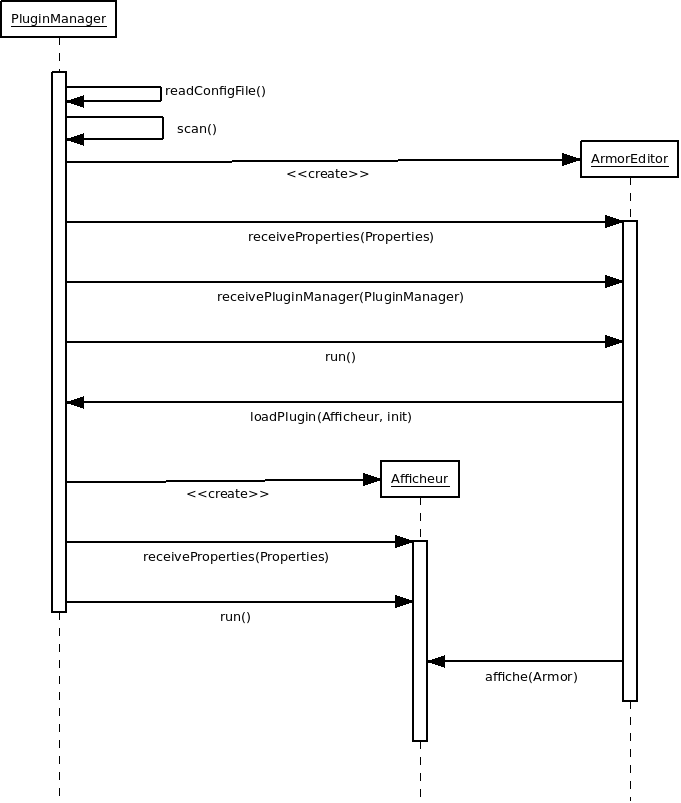
\includegraphics[width=\textwidth]{../figures/SeqLoadPlugin.png}
